% Created by tikzDevice version 0.10.1 on 2016-09-12 13:47:03
% !TEX encoding = UTF-8 Unicode
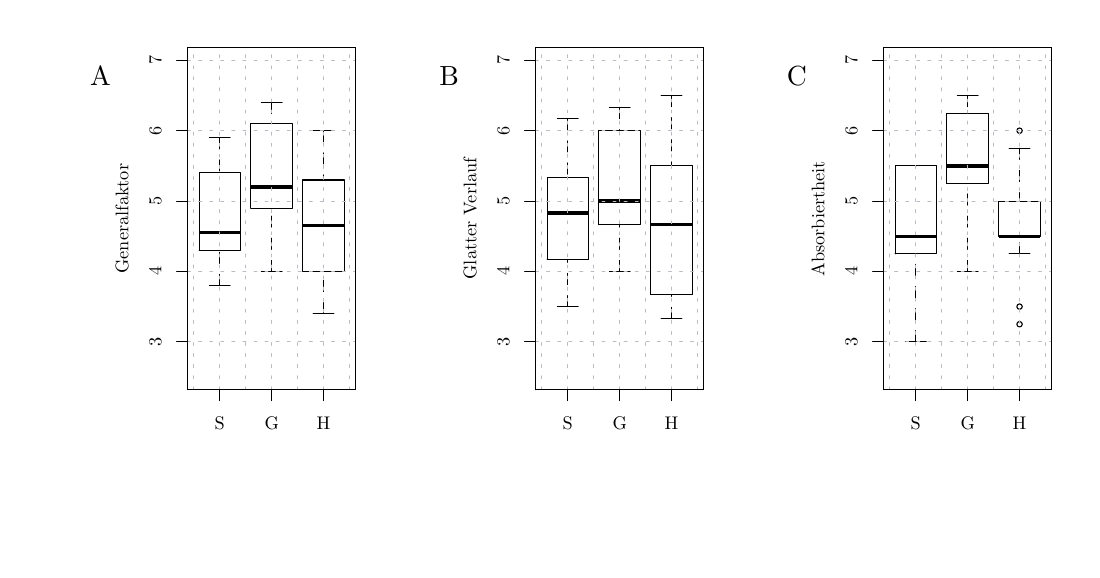
\begin{tikzpicture}[x=1pt,y=1pt]
\definecolor{fillColor}{RGB}{255,255,255}
\path[use as bounding box,fill=fillColor,fill opacity=0.00] (0,0) rectangle (377.25,188.62);
\begin{scope}
\path[clip] ( 57.82, 57.82) rectangle (118.52,181.40);
\definecolor{drawColor}{RGB}{0,0,0}

\path[draw=drawColor,line width= 1.2pt,line join=round] ( 61.94,114.52) -- ( 76.93,114.52);

\path[draw=drawColor,line width= 0.4pt,dash pattern=on 4pt off 4pt ,line join=round,line cap=round] ( 69.43, 95.45) -- ( 69.43,108.16);

\path[draw=drawColor,line width= 0.4pt,dash pattern=on 4pt off 4pt ,line join=round,line cap=round] ( 69.43,148.85) -- ( 69.43,136.14);

\path[draw=drawColor,line width= 0.4pt,line join=round,line cap=round] ( 65.69, 95.45) -- ( 73.18, 95.45);

\path[draw=drawColor,line width= 0.4pt,line join=round,line cap=round] ( 65.69,148.85) -- ( 73.18,148.85);

\path[draw=drawColor,line width= 0.4pt,line join=round,line cap=round] ( 61.94,108.16) --
	( 76.93,108.16) --
	( 76.93,136.14) --
	( 61.94,136.14) --
	( 61.94,108.16);

\path[draw=drawColor,line width= 1.2pt,line join=round] ( 80.67,131.05) -- ( 95.66,131.05);

\path[draw=drawColor,line width= 0.4pt,dash pattern=on 4pt off 4pt ,line join=round,line cap=round] ( 88.17,100.54) -- ( 88.17,123.42);

\path[draw=drawColor,line width= 0.4pt,dash pattern=on 4pt off 4pt ,line join=round,line cap=round] ( 88.17,161.56) -- ( 88.17,153.94);

\path[draw=drawColor,line width= 0.4pt,line join=round,line cap=round] ( 84.42,100.54) -- ( 91.92,100.54);

\path[draw=drawColor,line width= 0.4pt,line join=round,line cap=round] ( 84.42,161.56) -- ( 91.92,161.56);

\path[draw=drawColor,line width= 0.4pt,line join=round,line cap=round] ( 80.67,123.42) --
	( 95.66,123.42) --
	( 95.66,153.94) --
	( 80.67,153.94) --
	( 80.67,123.42);

\path[draw=drawColor,line width= 1.2pt,line join=round] ( 99.41,117.06) -- (114.40,117.06);

\path[draw=drawColor,line width= 0.4pt,dash pattern=on 4pt off 4pt ,line join=round,line cap=round] (106.91, 85.28) -- (106.91,100.54);

\path[draw=drawColor,line width= 0.4pt,dash pattern=on 4pt off 4pt ,line join=round,line cap=round] (106.91,151.39) -- (106.91,133.59);

\path[draw=drawColor,line width= 0.4pt,line join=round,line cap=round] (103.16, 85.28) -- (110.65, 85.28);

\path[draw=drawColor,line width= 0.4pt,line join=round,line cap=round] (103.16,151.39) -- (110.65,151.39);

\path[draw=drawColor,line width= 0.4pt,line join=round,line cap=round] ( 99.41,100.54) --
	(114.40,100.54) --
	(114.40,133.59) --
	( 99.41,133.59) --
	( 99.41,100.54);
\end{scope}
\begin{scope}
\path[clip] (  0.00,  0.00) rectangle (377.25,188.62);
\definecolor{drawColor}{RGB}{0,0,0}

\path[draw=drawColor,line width= 0.4pt,line join=round,line cap=round] ( 69.43, 57.82) -- (106.91, 57.82);

\path[draw=drawColor,line width= 0.4pt,line join=round,line cap=round] ( 69.43, 57.82) -- ( 69.43, 53.86);

\path[draw=drawColor,line width= 0.4pt,line join=round,line cap=round] ( 88.17, 57.82) -- ( 88.17, 53.86);

\path[draw=drawColor,line width= 0.4pt,line join=round,line cap=round] (106.91, 57.82) -- (106.91, 53.86);

\node[text=drawColor,anchor=base,inner sep=0pt, outer sep=0pt, scale=  0.66] at ( 69.43, 43.56) {S};

\node[text=drawColor,anchor=base,inner sep=0pt, outer sep=0pt, scale=  0.66] at ( 88.17, 43.56) {G};

\node[text=drawColor,anchor=base,inner sep=0pt, outer sep=0pt, scale=  0.66] at (106.91, 43.56) {H};

\path[draw=drawColor,line width= 0.4pt,line join=round,line cap=round] ( 57.82, 75.11) -- ( 57.82,176.82);

\path[draw=drawColor,line width= 0.4pt,line join=round,line cap=round] ( 57.82, 75.11) -- ( 53.86, 75.11);

\path[draw=drawColor,line width= 0.4pt,line join=round,line cap=round] ( 57.82,100.54) -- ( 53.86,100.54);

\path[draw=drawColor,line width= 0.4pt,line join=round,line cap=round] ( 57.82,125.96) -- ( 53.86,125.96);

\path[draw=drawColor,line width= 0.4pt,line join=round,line cap=round] ( 57.82,151.39) -- ( 53.86,151.39);

\path[draw=drawColor,line width= 0.4pt,line join=round,line cap=round] ( 57.82,176.82) -- ( 53.86,176.82);

\node[text=drawColor,rotate= 90.00,anchor=base,inner sep=0pt, outer sep=0pt, scale=  0.66] at ( 48.31, 75.11) {3};

\node[text=drawColor,rotate= 90.00,anchor=base,inner sep=0pt, outer sep=0pt, scale=  0.66] at ( 48.31,100.54) {4};

\node[text=drawColor,rotate= 90.00,anchor=base,inner sep=0pt, outer sep=0pt, scale=  0.66] at ( 48.31,125.96) {5};

\node[text=drawColor,rotate= 90.00,anchor=base,inner sep=0pt, outer sep=0pt, scale=  0.66] at ( 48.31,151.39) {6};

\node[text=drawColor,rotate= 90.00,anchor=base,inner sep=0pt, outer sep=0pt, scale=  0.66] at ( 48.31,176.82) {7};
\end{scope}
\begin{scope}
\path[clip] (  0.00,  0.00) rectangle (125.75,188.62);
\definecolor{drawColor}{RGB}{0,0,0}

\node[text=drawColor,rotate= 90.00,anchor=base,inner sep=0pt, outer sep=0pt, scale=  0.66] at ( 36.43,119.61) {Generalfaktor};
\end{scope}
\begin{scope}
\path[clip] (  0.00,  0.00) rectangle (377.25,188.62);
\definecolor{drawColor}{RGB}{0,0,0}

\path[draw=drawColor,line width= 0.4pt,line join=round,line cap=round] ( 57.82, 57.82) --
	(118.52, 57.82) --
	(118.52,181.40) --
	( 57.82,181.40) --
	( 57.82, 57.82);
\end{scope}
\begin{scope}
\path[clip] ( 57.82, 57.82) rectangle (118.52,181.40);
\definecolor{drawColor}{RGB}{186,187,194}

\path[draw=drawColor,line width= 0.4pt,dash pattern=on 1pt off 3pt ,line join=round,line cap=round] ( 60.06, 57.82) -- ( 60.06,181.40);

\path[draw=drawColor,line width= 0.4pt,dash pattern=on 1pt off 3pt ,line join=round,line cap=round] ( 69.43, 57.82) -- ( 69.43,181.40);

\path[draw=drawColor,line width= 0.4pt,dash pattern=on 1pt off 3pt ,line join=round,line cap=round] ( 78.80, 57.82) -- ( 78.80,181.40);

\path[draw=drawColor,line width= 0.4pt,dash pattern=on 1pt off 3pt ,line join=round,line cap=round] ( 88.17, 57.82) -- ( 88.17,181.40);

\path[draw=drawColor,line width= 0.4pt,dash pattern=on 1pt off 3pt ,line join=round,line cap=round] ( 97.54, 57.82) -- ( 97.54,181.40);

\path[draw=drawColor,line width= 0.4pt,dash pattern=on 1pt off 3pt ,line join=round,line cap=round] (106.91, 57.82) -- (106.91,181.40);

\path[draw=drawColor,line width= 0.4pt,dash pattern=on 1pt off 3pt ,line join=round,line cap=round] (116.27, 57.82) -- (116.27,181.40);

\path[draw=drawColor,line width= 0.4pt,dash pattern=on 1pt off 3pt ,line join=round,line cap=round] ( 57.82, 75.11) -- (118.52, 75.11);

\path[draw=drawColor,line width= 0.4pt,dash pattern=on 1pt off 3pt ,line join=round,line cap=round] ( 57.82,100.54) -- (118.52,100.54);

\path[draw=drawColor,line width= 0.4pt,dash pattern=on 1pt off 3pt ,line join=round,line cap=round] ( 57.82,125.96) -- (118.52,125.96);

\path[draw=drawColor,line width= 0.4pt,dash pattern=on 1pt off 3pt ,line join=round,line cap=round] ( 57.82,151.39) -- (118.52,151.39);

\path[draw=drawColor,line width= 0.4pt,dash pattern=on 1pt off 3pt ,line join=round,line cap=round] ( 57.82,176.82) -- (118.52,176.82);
\end{scope}
\begin{scope}
\path[clip] (  0.00,  0.00) rectangle (377.25,188.62);
\definecolor{drawColor}{RGB}{0,0,0}

\path[draw=drawColor,line width= 0.4pt,line join=round,line cap=round] ( 57.82, 57.82) --
	(118.52, 57.82) --
	(118.52,181.40) --
	( 57.82,181.40) --
	( 57.82, 57.82);

\node[text=drawColor,anchor=base east,inner sep=0pt, outer sep=0pt, scale=  1.00] at ( 30.10,167.82) {A};
\end{scope}
\begin{scope}
\path[clip] (183.57, 57.82) rectangle (244.27,181.40);
\definecolor{drawColor}{RGB}{0,0,0}

\path[draw=drawColor,line width= 1.2pt,line join=round] (187.69,121.64) -- (202.68,121.64);

\path[draw=drawColor,line width= 0.4pt,dash pattern=on 4pt off 4pt ,line join=round,line cap=round] (195.18, 87.82) -- (195.18,104.86);

\path[draw=drawColor,line width= 0.4pt,dash pattern=on 4pt off 4pt ,line join=round,line cap=round] (195.18,155.72) -- (195.18,134.36);

\path[draw=drawColor,line width= 0.4pt,line join=round,line cap=round] (191.44, 87.82) -- (198.93, 87.82);

\path[draw=drawColor,line width= 0.4pt,line join=round,line cap=round] (191.44,155.72) -- (198.93,155.72);

\path[draw=drawColor,line width= 0.4pt,line join=round,line cap=round] (187.69,104.86) --
	(202.68,104.86) --
	(202.68,134.36) --
	(187.69,134.36) --
	(187.69,104.86);

\path[draw=drawColor,line width= 1.2pt,line join=round] (206.42,125.96) -- (221.41,125.96);

\path[draw=drawColor,line width= 0.4pt,dash pattern=on 4pt off 4pt ,line join=round,line cap=round] (213.92,100.54) -- (213.92,117.45);

\path[draw=drawColor,line width= 0.4pt,dash pattern=on 4pt off 4pt ,line join=round,line cap=round] (213.92,159.78) -- (213.92,151.39);

\path[draw=drawColor,line width= 0.4pt,line join=round,line cap=round] (210.17,100.54) -- (217.67,100.54);

\path[draw=drawColor,line width= 0.4pt,line join=round,line cap=round] (210.17,159.78) -- (217.67,159.78);

\path[draw=drawColor,line width= 0.4pt,line join=round,line cap=round] (206.42,117.45) --
	(221.41,117.45) --
	(221.41,151.39) --
	(206.42,151.39) --
	(206.42,117.45);

\path[draw=drawColor,line width= 1.2pt,line join=round] (225.16,117.45) -- (240.15,117.45);

\path[draw=drawColor,line width= 0.4pt,dash pattern=on 4pt off 4pt ,line join=round,line cap=round] (232.66, 83.50) -- (232.66, 92.14);

\path[draw=drawColor,line width= 0.4pt,dash pattern=on 4pt off 4pt ,line join=round,line cap=round] (232.66,164.11) -- (232.66,138.68);

\path[draw=drawColor,line width= 0.4pt,line join=round,line cap=round] (228.91, 83.50) -- (236.40, 83.50);

\path[draw=drawColor,line width= 0.4pt,line join=round,line cap=round] (228.91,164.11) -- (236.40,164.11);

\path[draw=drawColor,line width= 0.4pt,line join=round,line cap=round] (225.16, 92.14) --
	(240.15, 92.14) --
	(240.15,138.68) --
	(225.16,138.68) --
	(225.16, 92.14);
\end{scope}
\begin{scope}
\path[clip] (  0.00,  0.00) rectangle (377.25,188.62);
\definecolor{drawColor}{RGB}{0,0,0}

\path[draw=drawColor,line width= 0.4pt,line join=round,line cap=round] (195.18, 57.82) -- (232.66, 57.82);

\path[draw=drawColor,line width= 0.4pt,line join=round,line cap=round] (195.18, 57.82) -- (195.18, 53.86);

\path[draw=drawColor,line width= 0.4pt,line join=round,line cap=round] (213.92, 57.82) -- (213.92, 53.86);

\path[draw=drawColor,line width= 0.4pt,line join=round,line cap=round] (232.66, 57.82) -- (232.66, 53.86);

\node[text=drawColor,anchor=base,inner sep=0pt, outer sep=0pt, scale=  0.66] at (195.18, 43.56) {S};

\node[text=drawColor,anchor=base,inner sep=0pt, outer sep=0pt, scale=  0.66] at (213.92, 43.56) {G};

\node[text=drawColor,anchor=base,inner sep=0pt, outer sep=0pt, scale=  0.66] at (232.66, 43.56) {H};

\path[draw=drawColor,line width= 0.4pt,line join=round,line cap=round] (183.57, 75.11) -- (183.57,176.82);

\path[draw=drawColor,line width= 0.4pt,line join=round,line cap=round] (183.57, 75.11) -- (179.61, 75.11);

\path[draw=drawColor,line width= 0.4pt,line join=round,line cap=round] (183.57,100.54) -- (179.61,100.54);

\path[draw=drawColor,line width= 0.4pt,line join=round,line cap=round] (183.57,125.96) -- (179.61,125.96);

\path[draw=drawColor,line width= 0.4pt,line join=round,line cap=round] (183.57,151.39) -- (179.61,151.39);

\path[draw=drawColor,line width= 0.4pt,line join=round,line cap=round] (183.57,176.82) -- (179.61,176.82);

\node[text=drawColor,rotate= 90.00,anchor=base,inner sep=0pt, outer sep=0pt, scale=  0.66] at (174.06, 75.11) {3};

\node[text=drawColor,rotate= 90.00,anchor=base,inner sep=0pt, outer sep=0pt, scale=  0.66] at (174.06,100.54) {4};

\node[text=drawColor,rotate= 90.00,anchor=base,inner sep=0pt, outer sep=0pt, scale=  0.66] at (174.06,125.96) {5};

\node[text=drawColor,rotate= 90.00,anchor=base,inner sep=0pt, outer sep=0pt, scale=  0.66] at (174.06,151.39) {6};

\node[text=drawColor,rotate= 90.00,anchor=base,inner sep=0pt, outer sep=0pt, scale=  0.66] at (174.06,176.82) {7};
\end{scope}
\begin{scope}
\path[clip] (125.75,  0.00) rectangle (251.50,188.62);
\definecolor{drawColor}{RGB}{0,0,0}

\node[text=drawColor,rotate= 90.00,anchor=base,inner sep=0pt, outer sep=0pt, scale=  0.66] at (162.18,119.61) {Glatter Verlauf};
\end{scope}
\begin{scope}
\path[clip] (  0.00,  0.00) rectangle (377.25,188.62);
\definecolor{drawColor}{RGB}{0,0,0}

\path[draw=drawColor,line width= 0.4pt,line join=round,line cap=round] (183.57, 57.82) --
	(244.27, 57.82) --
	(244.27,181.40) --
	(183.57,181.40) --
	(183.57, 57.82);
\end{scope}
\begin{scope}
\path[clip] (183.57, 57.82) rectangle (244.27,181.40);
\definecolor{drawColor}{RGB}{186,187,194}

\path[draw=drawColor,line width= 0.4pt,dash pattern=on 1pt off 3pt ,line join=round,line cap=round] (185.81, 57.82) -- (185.81,181.40);

\path[draw=drawColor,line width= 0.4pt,dash pattern=on 1pt off 3pt ,line join=round,line cap=round] (195.18, 57.82) -- (195.18,181.40);

\path[draw=drawColor,line width= 0.4pt,dash pattern=on 1pt off 3pt ,line join=round,line cap=round] (204.55, 57.82) -- (204.55,181.40);

\path[draw=drawColor,line width= 0.4pt,dash pattern=on 1pt off 3pt ,line join=round,line cap=round] (213.92, 57.82) -- (213.92,181.40);

\path[draw=drawColor,line width= 0.4pt,dash pattern=on 1pt off 3pt ,line join=round,line cap=round] (223.29, 57.82) -- (223.29,181.40);

\path[draw=drawColor,line width= 0.4pt,dash pattern=on 1pt off 3pt ,line join=round,line cap=round] (232.66, 57.82) -- (232.66,181.40);

\path[draw=drawColor,line width= 0.4pt,dash pattern=on 1pt off 3pt ,line join=round,line cap=round] (242.02, 57.82) -- (242.02,181.40);

\path[draw=drawColor,line width= 0.4pt,dash pattern=on 1pt off 3pt ,line join=round,line cap=round] (183.57, 75.11) -- (244.27, 75.11);

\path[draw=drawColor,line width= 0.4pt,dash pattern=on 1pt off 3pt ,line join=round,line cap=round] (183.57,100.54) -- (244.27,100.54);

\path[draw=drawColor,line width= 0.4pt,dash pattern=on 1pt off 3pt ,line join=round,line cap=round] (183.57,125.96) -- (244.27,125.96);

\path[draw=drawColor,line width= 0.4pt,dash pattern=on 1pt off 3pt ,line join=round,line cap=round] (183.57,151.39) -- (244.27,151.39);

\path[draw=drawColor,line width= 0.4pt,dash pattern=on 1pt off 3pt ,line join=round,line cap=round] (183.57,176.82) -- (244.27,176.82);
\end{scope}
\begin{scope}
\path[clip] (  0.00,  0.00) rectangle (377.25,188.62);
\definecolor{drawColor}{RGB}{0,0,0}

\path[draw=drawColor,line width= 0.4pt,line join=round,line cap=round] (183.57, 57.82) --
	(244.27, 57.82) --
	(244.27,181.40) --
	(183.57,181.40) --
	(183.57, 57.82);

\node[text=drawColor,anchor=base east,inner sep=0pt, outer sep=0pt, scale=  1.00] at (155.85,167.82) {B};
\end{scope}
\begin{scope}
\path[clip] (309.32, 57.82) rectangle (370.02,181.40);
\definecolor{drawColor}{RGB}{0,0,0}

\path[draw=drawColor,line width= 1.2pt,line join=round] (313.44,113.25) -- (328.43,113.25);

\path[draw=drawColor,line width= 0.4pt,dash pattern=on 4pt off 4pt ,line join=round,line cap=round] (320.93, 75.11) -- (320.93,106.89);

\path[draw=drawColor,line width= 0.4pt,dash pattern=on 4pt off 4pt ,line join=round,line cap=round] (320.93,138.68) -- (320.93,138.68);

\path[draw=drawColor,line width= 0.4pt,line join=round,line cap=round] (317.19, 75.11) -- (324.68, 75.11);

\path[draw=drawColor,line width= 0.4pt,line join=round,line cap=round] (317.19,138.68) -- (324.68,138.68);

\path[draw=drawColor,line width= 0.4pt,line join=round,line cap=round] (313.44,106.89) --
	(328.43,106.89) --
	(328.43,138.68) --
	(313.44,138.68) --
	(313.44,106.89);

\path[draw=drawColor,line width= 1.2pt,line join=round] (332.17,138.68) -- (347.16,138.68);

\path[draw=drawColor,line width= 0.4pt,dash pattern=on 4pt off 4pt ,line join=round,line cap=round] (339.67,100.54) -- (339.67,132.32);

\path[draw=drawColor,line width= 0.4pt,dash pattern=on 4pt off 4pt ,line join=round,line cap=round] (339.67,164.11) -- (339.67,157.75);

\path[draw=drawColor,line width= 0.4pt,line join=round,line cap=round] (335.92,100.54) -- (343.42,100.54);

\path[draw=drawColor,line width= 0.4pt,line join=round,line cap=round] (335.92,164.11) -- (343.42,164.11);

\path[draw=drawColor,line width= 0.4pt,line join=round,line cap=round] (332.17,132.32) --
	(347.16,132.32) --
	(347.16,157.75) --
	(332.17,157.75) --
	(332.17,132.32);

\path[draw=drawColor,line width= 1.2pt,line join=round] (350.91,113.25) -- (365.90,113.25);

\path[draw=drawColor,line width= 0.4pt,dash pattern=on 4pt off 4pt ,line join=round,line cap=round] (358.41,106.89) -- (358.41,113.25);

\path[draw=drawColor,line width= 0.4pt,dash pattern=on 4pt off 4pt ,line join=round,line cap=round] (358.41,145.04) -- (358.41,125.96);

\path[draw=drawColor,line width= 0.4pt,line join=round,line cap=round] (354.66,106.89) -- (362.15,106.89);

\path[draw=drawColor,line width= 0.4pt,line join=round,line cap=round] (354.66,145.04) -- (362.15,145.04);

\path[draw=drawColor,line width= 0.4pt,line join=round,line cap=round] (350.91,113.25) --
	(365.90,113.25) --
	(365.90,125.96) --
	(350.91,125.96) --
	(350.91,113.25);

\path[draw=drawColor,line width= 0.4pt,line join=round,line cap=round] (358.41,151.39) circle (  0.98);

\path[draw=drawColor,line width= 0.4pt,line join=round,line cap=round] (358.41, 81.46) circle (  0.98);

\path[draw=drawColor,line width= 0.4pt,line join=round,line cap=round] (358.41, 87.82) circle (  0.98);
\end{scope}
\begin{scope}
\path[clip] (  0.00,  0.00) rectangle (377.25,188.62);
\definecolor{drawColor}{RGB}{0,0,0}

\path[draw=drawColor,line width= 0.4pt,line join=round,line cap=round] (320.93, 57.82) -- (358.41, 57.82);

\path[draw=drawColor,line width= 0.4pt,line join=round,line cap=round] (320.93, 57.82) -- (320.93, 53.86);

\path[draw=drawColor,line width= 0.4pt,line join=round,line cap=round] (339.67, 57.82) -- (339.67, 53.86);

\path[draw=drawColor,line width= 0.4pt,line join=round,line cap=round] (358.41, 57.82) -- (358.41, 53.86);

\node[text=drawColor,anchor=base,inner sep=0pt, outer sep=0pt, scale=  0.66] at (320.93, 43.56) {S};

\node[text=drawColor,anchor=base,inner sep=0pt, outer sep=0pt, scale=  0.66] at (339.67, 43.56) {G};

\node[text=drawColor,anchor=base,inner sep=0pt, outer sep=0pt, scale=  0.66] at (358.41, 43.56) {H};

\path[draw=drawColor,line width= 0.4pt,line join=round,line cap=round] (309.32, 75.11) -- (309.32,176.82);

\path[draw=drawColor,line width= 0.4pt,line join=round,line cap=round] (309.32, 75.11) -- (305.36, 75.11);

\path[draw=drawColor,line width= 0.4pt,line join=round,line cap=round] (309.32,100.54) -- (305.36,100.54);

\path[draw=drawColor,line width= 0.4pt,line join=round,line cap=round] (309.32,125.96) -- (305.36,125.96);

\path[draw=drawColor,line width= 0.4pt,line join=round,line cap=round] (309.32,151.39) -- (305.36,151.39);

\path[draw=drawColor,line width= 0.4pt,line join=round,line cap=round] (309.32,176.82) -- (305.36,176.82);

\node[text=drawColor,rotate= 90.00,anchor=base,inner sep=0pt, outer sep=0pt, scale=  0.66] at (299.81, 75.11) {3};

\node[text=drawColor,rotate= 90.00,anchor=base,inner sep=0pt, outer sep=0pt, scale=  0.66] at (299.81,100.54) {4};

\node[text=drawColor,rotate= 90.00,anchor=base,inner sep=0pt, outer sep=0pt, scale=  0.66] at (299.81,125.96) {5};

\node[text=drawColor,rotate= 90.00,anchor=base,inner sep=0pt, outer sep=0pt, scale=  0.66] at (299.81,151.39) {6};

\node[text=drawColor,rotate= 90.00,anchor=base,inner sep=0pt, outer sep=0pt, scale=  0.66] at (299.81,176.82) {7};
\end{scope}
\begin{scope}
\path[clip] (251.50,  0.00) rectangle (377.25,188.62);
\definecolor{drawColor}{RGB}{0,0,0}

\node[text=drawColor,rotate= 90.00,anchor=base,inner sep=0pt, outer sep=0pt, scale=  0.66] at (287.93,119.61) {Absorbiertheit};
\end{scope}
\begin{scope}
\path[clip] (  0.00,  0.00) rectangle (377.25,188.62);
\definecolor{drawColor}{RGB}{0,0,0}

\path[draw=drawColor,line width= 0.4pt,line join=round,line cap=round] (309.32, 57.82) --
	(370.02, 57.82) --
	(370.02,181.40) --
	(309.32,181.40) --
	(309.32, 57.82);
\end{scope}
\begin{scope}
\path[clip] (309.32, 57.82) rectangle (370.02,181.40);
\definecolor{drawColor}{RGB}{186,187,194}

\path[draw=drawColor,line width= 0.4pt,dash pattern=on 1pt off 3pt ,line join=round,line cap=round] (311.56, 57.82) -- (311.56,181.40);

\path[draw=drawColor,line width= 0.4pt,dash pattern=on 1pt off 3pt ,line join=round,line cap=round] (320.93, 57.82) -- (320.93,181.40);

\path[draw=drawColor,line width= 0.4pt,dash pattern=on 1pt off 3pt ,line join=round,line cap=round] (330.30, 57.82) -- (330.30,181.40);

\path[draw=drawColor,line width= 0.4pt,dash pattern=on 1pt off 3pt ,line join=round,line cap=round] (339.67, 57.82) -- (339.67,181.40);

\path[draw=drawColor,line width= 0.4pt,dash pattern=on 1pt off 3pt ,line join=round,line cap=round] (349.04, 57.82) -- (349.04,181.40);

\path[draw=drawColor,line width= 0.4pt,dash pattern=on 1pt off 3pt ,line join=round,line cap=round] (358.41, 57.82) -- (358.41,181.40);

\path[draw=drawColor,line width= 0.4pt,dash pattern=on 1pt off 3pt ,line join=round,line cap=round] (367.77, 57.82) -- (367.77,181.40);

\path[draw=drawColor,line width= 0.4pt,dash pattern=on 1pt off 3pt ,line join=round,line cap=round] (309.32, 75.11) -- (370.02, 75.11);

\path[draw=drawColor,line width= 0.4pt,dash pattern=on 1pt off 3pt ,line join=round,line cap=round] (309.32,100.54) -- (370.02,100.54);

\path[draw=drawColor,line width= 0.4pt,dash pattern=on 1pt off 3pt ,line join=round,line cap=round] (309.32,125.96) -- (370.02,125.96);

\path[draw=drawColor,line width= 0.4pt,dash pattern=on 1pt off 3pt ,line join=round,line cap=round] (309.32,151.39) -- (370.02,151.39);

\path[draw=drawColor,line width= 0.4pt,dash pattern=on 1pt off 3pt ,line join=round,line cap=round] (309.32,176.82) -- (370.02,176.82);
\end{scope}
\begin{scope}
\path[clip] (  0.00,  0.00) rectangle (377.25,188.62);
\definecolor{drawColor}{RGB}{0,0,0}

\path[draw=drawColor,line width= 0.4pt,line join=round,line cap=round] (309.32, 57.82) --
	(370.02, 57.82) --
	(370.02,181.40) --
	(309.32,181.40) --
	(309.32, 57.82);

\node[text=drawColor,anchor=base east,inner sep=0pt, outer sep=0pt, scale=  1.00] at (281.60,167.82) {C};
\end{scope}
\end{tikzpicture}
